%%  EE7218 / EC7207 — High Performance Computing — Analysis Report
%%  Topic: Parallel protein secondary structure prediction on CB513
%%  Build: pdflatex analysis_report.tex  (run twice for refs)

\documentclass[11pt,a4paper]{article}

\usepackage[margin=1in,headheight=22pt]{geometry}
\usepackage[utf8]{inputenc}
\usepackage[T1]{fontenc}
\usepackage{lmodern}
\usepackage{microtype}
\usepackage{amsmath,amssymb}
\usepackage{graphicx}
\usepackage{booktabs}
\usepackage{array}
\usepackage{tabularx}
\usepackage{multirow}
\usepackage{caption}
\usepackage{listings}
\usepackage{xcolor}
\usepackage{tikz}
\usetikzlibrary{positioning,arrows.meta,shapes.geometric,fit,backgrounds}
\usepackage[hidelinks]{hyperref}
\usepackage{float}
\usepackage{enumitem}
\usepackage{fancyhdr}
\usepackage{titlesec}

\definecolor{ReportBlue}{HTML}{1D4ED8}
\definecolor{ReportSlate}{HTML}{334155}
\definecolor{ReportRule}{HTML}{CBD5E1}

\lstset{
  basicstyle=\ttfamily\footnotesize,
  breaklines=true,
  frame=single,
  backgroundcolor=\color{gray!8},
  columns=fullflexible,
  keepspaces=true,
  showstringspaces=false,
}

\captionsetup{
  font=small,
  labelfont=bf,
  justification=justified,
  singlelinecheck=false,
  skip=6pt
}
\setlist{itemsep=2pt,topsep=4pt,leftmargin=1.5em}
\setlength{\parskip}{0.35em}
\setlength{\parindent}{0pt}
\renewcommand{\arraystretch}{1.12}
\titleformat{\section}
  {\Large\bfseries\color{ReportSlate}}
  {\thesection}{0.8em}{}
\titleformat{\subsection}
  {\large\bfseries\color{ReportSlate}}
  {\thesubsection}{0.8em}{}
\titlespacing*{\section}{0pt}{1.4em}{0.65em}
\titlespacing*{\subsection}{0pt}{1.0em}{0.45em}

\pagestyle{fancy}
\fancyhf{}
\cfoot{\small\thepage}
\renewcommand{\headrulewidth}{0pt}

\graphicspath{{figures/}{../../plots/}{plots/}{../diagrams/png/}}

\newcommand{\reporttitle}{Parallel Training of an MLP Neural Network for Protein Secondary Structure Classification}
\newcommand{\reportsubtitle}{A CB513 Evaluation Using Serial, OpenMP, POSIX Threads, MPI, Hybrid MPI+OpenMP, and CUDA}
\newcommand{\reportcourse}{EE7218 / EC7207 --- High Performance Computing Project}
\newcommand{\reportgroup}{Group 36}
\newcommand{\reportdate}{\today}

\hypersetup{
  pdftitle={\reporttitle},
  pdfauthor={Group 36},
  pdfsubject={High Performance Computing Project Report}
}

\begin{document}
\pagenumbering{roman}
\hypersetup{pageanchor=false}
\begin{titlepage}
  \thispagestyle{empty}
  \centering
  
\includegraphics[width=3cm]{Logo.jpeg}\par\vspace{0.9cm}
  {\LARGE\bfseries Department of Electrical and Information Engineering\par}\vspace{0.35cm}
  {\Large\bfseries University of Ruhuna\par}\vspace{1.4cm}

  {\Large\bfseries \reportcourse\par}\vspace{1.4cm}

  {\LARGE\bfseries \reporttitle\par}\vspace{0.45cm}
  {\large\color{ReportSlate}\reportsubtitle\par}\vspace{0.85cm}
  {\color{ReportBlue}\rule{0.72\textwidth}{1.2pt}\par}\vspace{0.85cm}

  {\Large\bfseries \reportgroup\par}\vspace{0.35cm}
  {\normalsize
    EG/2021/4684 \quad MUNSIF M.F.A.\\
    EG/2021/4685 \quad MUTHUKUMARI H.M.S.\\
    EG/2021/4686 \quad NADHA M.J.\par}

  \vspace{1.4cm}
  {\large \reportdate\par}

  \vfill
  Department of Electrical and Information Engineering\\
  University of Ruhuna
\end{titlepage}

\clearpage
\hypersetup{pageanchor=true}
\setcounter{page}{1}
\thispagestyle{plain}
\tableofcontents
\clearpage
\pagenumbering{arabic}

%%======================================================================
\section{Introduction and Motivation}\label{sec:intro}

Protein secondary-structure prediction assigns each residue of a protein
sequence to one of three classes: $\alpha$-helix~(H), $\beta$-sheet~(E), or
coil~(C). It is an enabling step for downstream tertiary-structure analysis
and drug design, and the classical approach is to train a neural network
over a sliding window of residues centred on the target
residue~\cite{rost1993,zhong2007}. Zhong~et~al.~\cite{zhong2007} showed on
early multi-core Intel hardware that the training of such a network
parallelises well using OpenMP or POSIX threads, obtaining speedups close
to the core count. In this project we repeat that experiment on modern
hardware \emph{and} extend the parallelisation strategies to distributed
memory (MPI), a hybrid shared/distributed scheme, and GPU acceleration
(CUDA).

The report focuses on three evaluation questions: how each parallel
programming concept is applied to the neural-network training loop, whether
the parallel versions preserve the serial prediction accuracy, and how
runtime changes as the thread count, rank count, hybrid layout, or CUDA
batch size is varied.

%%======================================================================
\section{Dataset and Preprocessing}\label{sec:data}

We use the CB513 benchmark of Cuff \& Barton~\cite{cuff1999}, a curated
set of $513$ non-homologous protein domains (${\sim}84\,000$~residues). The
processing pipeline is deterministic under a fixed seed:

\begin{enumerate}[noitemsep,topsep=2pt]
  \item \textbf{Download} --- fetches the canonical distribution tarball.
  \item \textbf{Parse} --- extracts \texttt{(protein\_id, residue,
        8-state-label)} tuples from the raw \texttt{.all} files.
  \item \textbf{8$\to$3 collapse} --- DSSP labels are collapsed to Q3
        using the mapping described in~\cite{zhong2007}:
        \(H,G,I \to H\); \(B,E \to E\); everything else $\to C$.
  \item \textbf{Sliding window} of size~$13$ with flat-edge padding,
        one-hot encoded over the $20$ amino-acid classes, giving an
        input vector of dimension \(20 \times 13 = 260\).
  \item \textbf{Split} --- fixed 70/15/15 train/validation/test; split indices
        are persisted with the processed dataset metadata.
  \item \textbf{Binary persistence} --- the final tensors are serialised
        under the processed CB513 binary-data directory for fast loading.
\end{enumerate}

\begin{figure}[H]
  \centering
  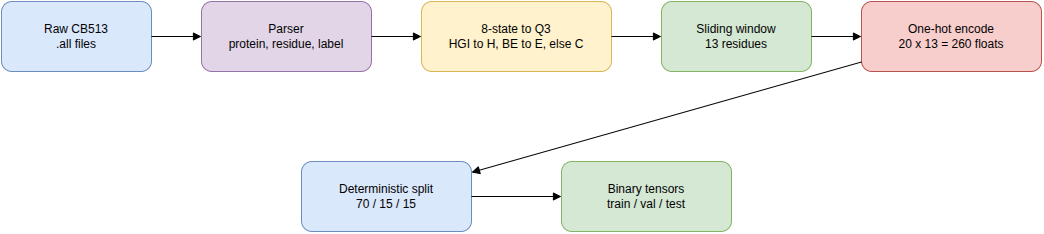
\includegraphics[width=\textwidth]{01_preprocessing_pipeline.png}
  \caption{Preprocessing workflow. Raw CB513 files are parsed, mapped from
  eight DSSP classes to three Q3 classes, converted to sliding-window
  one-hot features, split, and persisted as binary tensors for all
  training variants.}
  \label{fig:preprocess_workflow}
\end{figure}

Final sample counts are summarised in Table~\ref{tab:data}. The class
distribution is approximately $33\%\,H$ / $22\%\,E$ / $45\%\,C$ across every
split, consistent with published statistics for CB513.

\begin{table}[H]
  \centering
  \caption{Dataset splits after preprocessing.}\label{tab:data}
  \begin{tabular*}{0.88\textwidth}{@{\extracolsep{\fill}}lrrrr@{}}
    \toprule
    Split & Proteins & Residues (samples) & Feature dim & Classes\\
    \midrule
    train & 359 & 58\,363 & 260 & 3\\
    val   &  77 & 13\,064 & 260 & 3\\
    test  &  77 & 12\,692 & 260 & 3\\
    \bottomrule
  \end{tabular*}
\end{table}

%%======================================================================
\section{Serial Model and the \texorpdfstring{$\mathrm{Q}_3$}{Q3} Metric}
\label{sec:serial}

The model is a two-hidden-layer MLP:
\[
  \text{Input}(260)\to\text{Dense}(H_1)\to\text{ReLU}
  \to\text{Dense}(H_2)\to\text{ReLU}\to\text{Dense}(3)\to\text{Softmax}.
\]
Loss is cross-entropy fused with softmax for a numerically stable
backward pass:
\[
  \frac{\partial L}{\partial z_3} = p - \mathbf{1}_{y_{\text{true}}},
\]
where $p=\mathrm{softmax}(z_3)$ and $\mathbf{1}_{y}$ is the one-hot
encoding of the true label. Optimisation uses mini-batch SGD with an
optional step-decay learning rate. The reference configuration used for
every comparison run is
\begin{center}
  \(H_1=256\), \(H_2=128\), \(\mathrm{epochs}=80\), \(\mathrm{batch}=64\),
  \(\mathrm{lr}=0.01\), \(\mathrm{seed}=42\).
\end{center}

\begin{figure}[H]
  \centering
  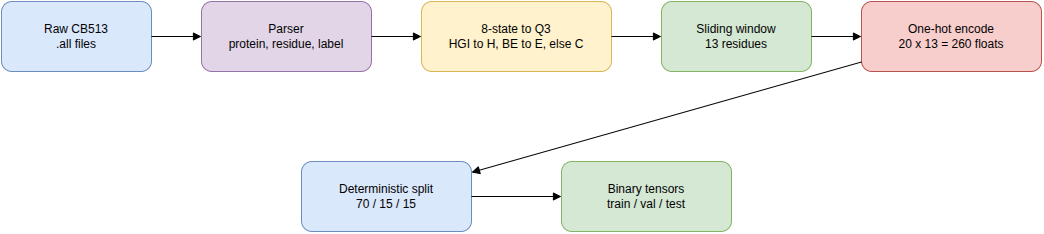
\includegraphics[width=\textwidth]{02_serial_training_loop.png}
  \caption{Serial training-loop workflow. Each mini-batch performs forward
  propagation, back-propagation, one SGD update, validation logging, and
  final test evaluation.}
  \label{fig:serial_workflow}
\end{figure}

The $\mathrm{Q}_3$ metric, following Eq.~(19) of Zhong~et~al., is
\begin{equation}\label{eq:q3}
  \mathrm{Q}_3 \;=\;
  \frac{N^{\text{correct}}_H + N^{\text{correct}}_E + N^{\text{correct}}_C}%
       {N_{\text{total}}} \times 100\,\%.
\end{equation}
This project is a three-class classification problem, so Q3 accuracy is
the appropriate serial-vs-parallel accuracy metric rather than a regression
metric such as RMSE.

On the reference 80-epoch run (single CPU worker, GCC with \texttt{-O3
-march=native}) the serial baseline achieves
\[
  \boxed{\text{test}\ \mathrm{Q}_3 = 59.28\,\%} \qquad
  \text{total training time}=236.8\,\mathrm{s}.
\]
All parallel variants are validated against this reference.

%%======================================================================
\section{Parallel Designs}\label{sec:designs}

Every variant trains the same MLP and uses the same mini-batch SGD
semantics. The variants differ only in how the mini-batch is partitioned
among workers and how their per-worker gradients are combined before the
SGD update. A single rule holds across all designs:

\begin{quote}
\textit{Model weights are \textbf{read-only} during the parallel region.
Each worker accumulates gradients into a \textbf{private} buffer; a
reduction sums these; a single SGD update is then applied. This removes
all locking on the weight matrices.}
\end{quote}

Formally, denote the model parameters by $\theta$, the learning rate by
$\eta$, the mini-batch size by $B$, and the number of parallel workers by
$W$. Every variant in this report instantiates the same parallel
mini-batch SGD template:
\begin{equation}\label{eq:parallel-sgd}
\begin{aligned}
&\textbf{for}\ \mathrm{epoch}=1,\dots,E:\\
&\quad \mathrm{shuffle}(\mathrm{train\_indices})\\
&\quad \textbf{for each mini-batch}\ \mathcal{B}\subset\{1,\dots,N\},\ |\mathcal{B}|=B:\\
&\qquad \mathcal{B}=\bigsqcup_{w=1}^{W}\mathcal{B}_{w}\ \text{(disjoint per-worker slices)}\\
&\qquad \mathbf{g}_{w}\;=\;\sum_{i\in\mathcal{B}_{w}}\nabla_{\theta}\,\ell\bigl(x_{i},y_{i};\theta\bigr)
       \quad\text{in parallel; $\theta$ read-only}\\
&\qquad \mathbf{g}\;=\;\mathop{\textstyle\bigoplus}_{w=1}^{W}\mathbf{g}_{w}
       \quad\text{(reduction; mechanism is variant-specific)}\\
&\qquad \theta\;\leftarrow\;\theta-\tfrac{\eta}{B}\,\mathbf{g}
\end{aligned}
\end{equation}
The first three lines and the final SGD update are identical across
variants; the per-worker gradient slice and the reduction
$\bigoplus_{w}\mathbf{g}_{w}$ are what each parallelisation specialises.
The next five subsections describe exactly how each variant realises the
reduction step.

\subsection{OpenMP}\label{sec:openmp}

The OpenMP variant uses shared-memory data parallelism. The model weights
are shared but read-only while a mini-batch is split across $T$ threads.
A \verb|#pragma omp parallel for schedule(static)| over the mini-batch
indices fans the work out to the team, each thread accumulates into a
thread-private \texttt{MLPGrad} struct, and an implicit barrier at the
end of the parallel region serialises the post-loop reduction. The master
thread (thread 0) then performs the gradient sum and applies a single SGD
update. Concretely, the reduction step of
Equation~\eqref{eq:parallel-sgd} is realised as
\begin{equation}\label{eq:omp-reduce}
  \mathbf{g}\;=\;\sum_{w=0}^{T-1}\mathbf{g}_{w}
  \qquad\text{(serial post-barrier reduce in shared memory)}.
\end{equation}

\begin{figure}[H]
  \centering
  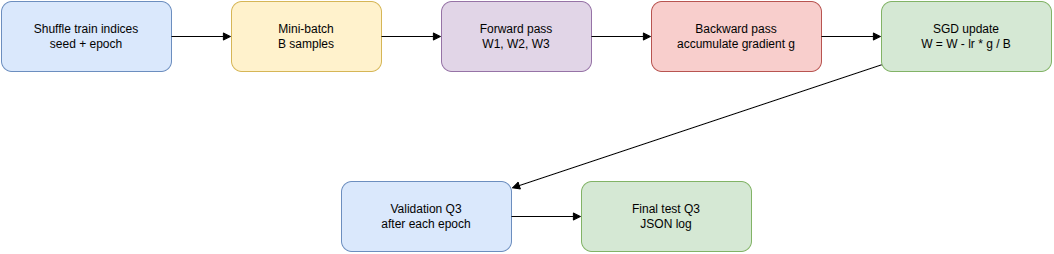
\includegraphics[width=\textwidth]{03_openmp_shared_memory.png}
  \caption{OpenMP shared-memory workflow. Model weights are shared and
  read-only during the parallel region; each thread writes only to its own
  private gradient buffer before the master performs one reduction and SGD
  update.}
  \label{fig:omp}
\end{figure}

\verb|schedule(static)| gives every thread a contiguous, size-balanced
slice and avoids work-stealing overhead. Runtime placement is pinned
with \verb|OMP_PROC_BIND=true| \verb|OMP_PLACES=cores|, which on the
i9-14900K keeps each thread on its own physical core and lets
first-touch allocation localise the gradient buffer to that core for
the whole epoch.

\subsection{POSIX Threads}\label{sec:pthreads}

The POSIX Threads variant implements the same shared-memory idea
manually, with full control of the thread-pool lifecycle. The master
spawns $T-1$ worker threads \emph{once} at the start of training and
keeps them alive for every mini-batch in the run, avoiding the
\verb|pthread_create|/\verb|pthread_join| cost that a naive
fork-per-batch design would pay each step. Two barriers gate the inner
loop: \verb|bar_start| releases all workers onto the current mini-batch,
they each accumulate into a thread-local gradient slot, \verb|bar_done|
waits for all of them, and the master then sums the slots and applies
the SGD update. The reduction therefore takes the same algebraic form as
Equation~\eqref{eq:omp-reduce},
\begin{equation}\label{eq:pth-reduce}
  \mathbf{g}\;=\;\sum_{w=0}^{T-1}\mathbf{g}_{w}
  \qquad\text{(master sum, after \texttt{bar\_done})},
\end{equation}
but the synchronisation primitive is explicit rather than implicit.

\begin{figure}[H]
  \centering
  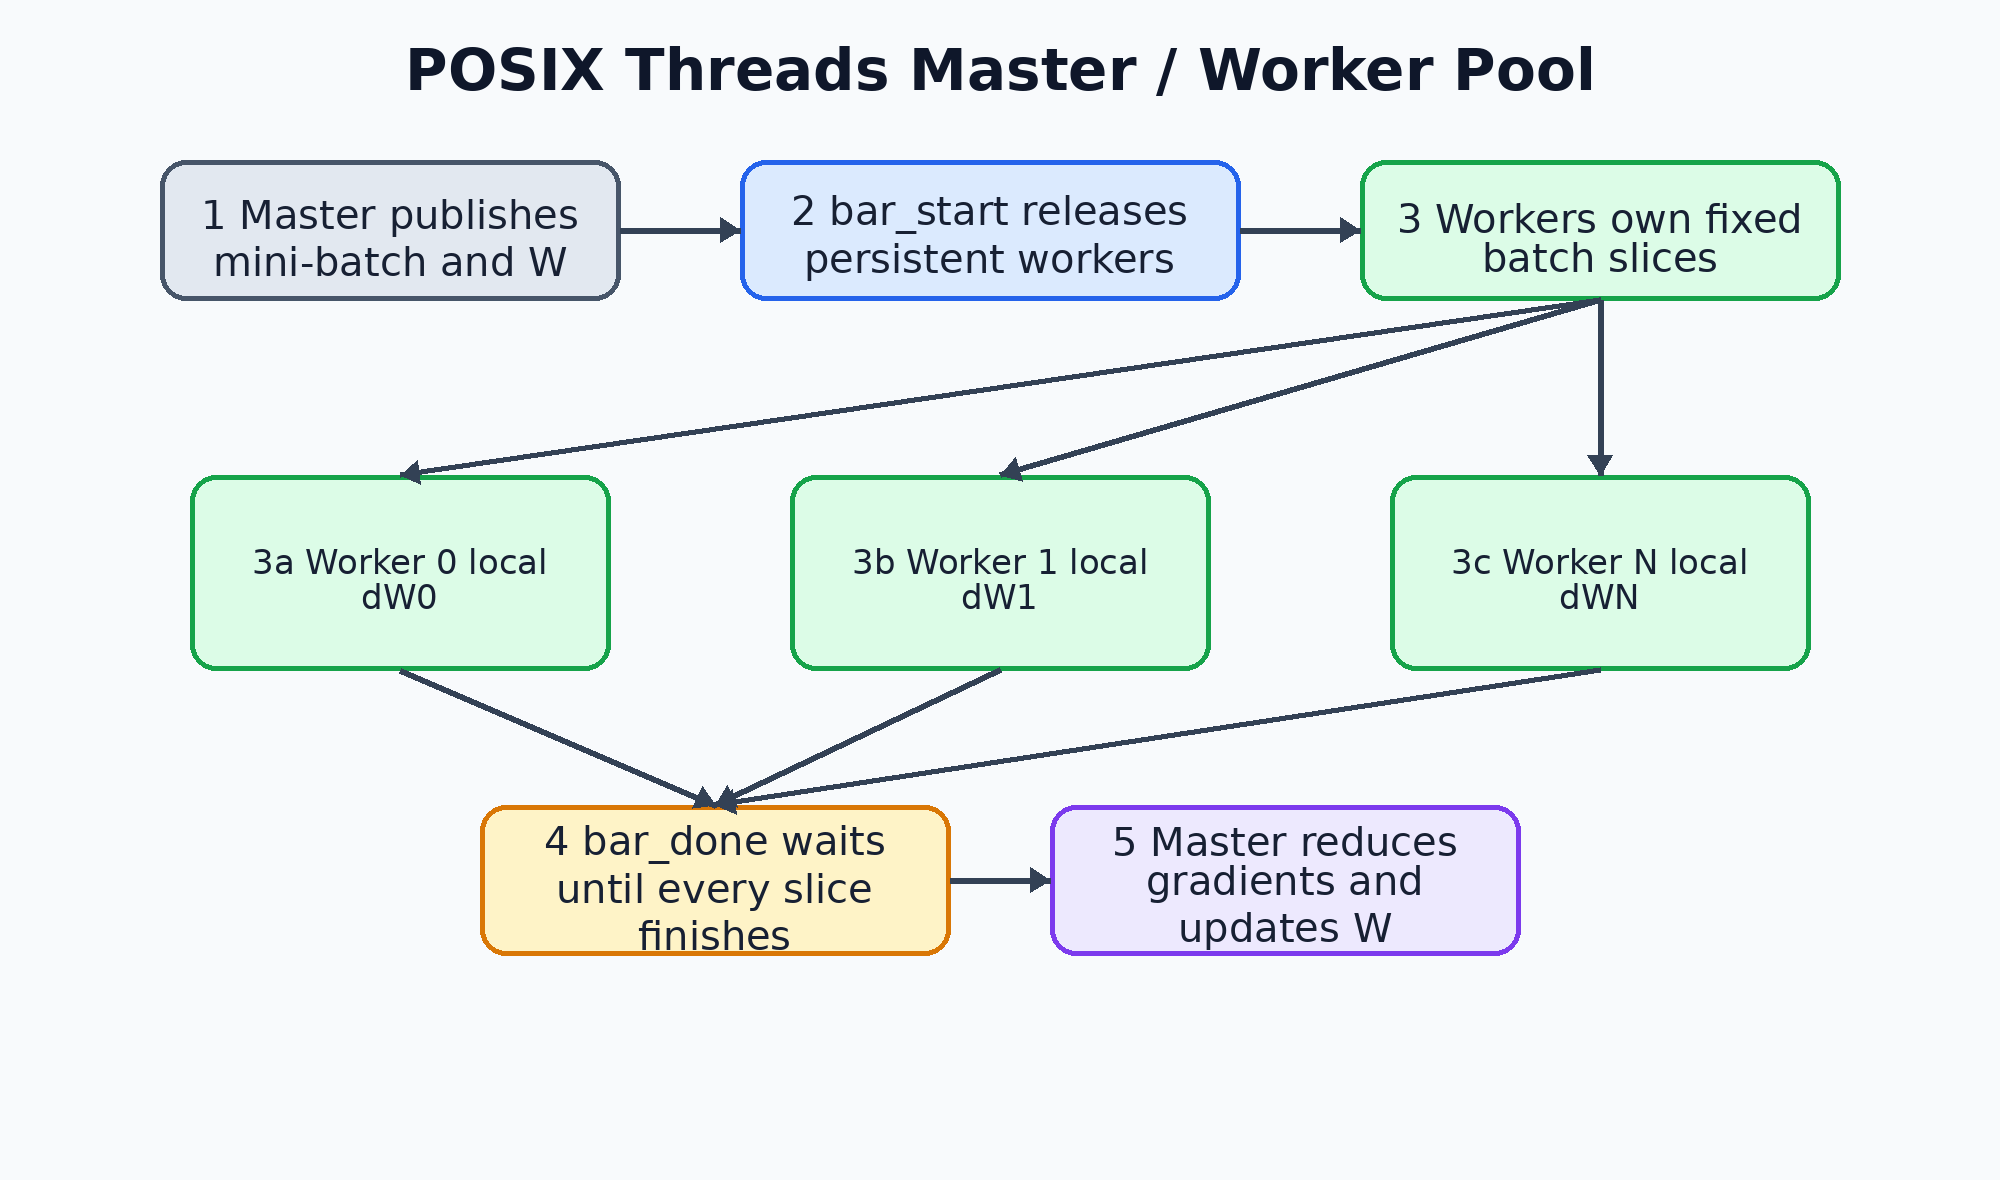
\includegraphics[width=\textwidth]{04_pthreads_master_worker.png}
  \caption{Pthreads master/worker workflow. Workers live for the entire
  run; two barriers gate each mini-batch, and the master performs the
  gradient reduction and SGD update after all workers finish their slices.}
  \label{fig:pth}
\end{figure}

Shutdown is clean: the master sets \verb|exit_flag|, trips
\verb|bar_start| once more, and each worker is joined. The persistent
pool keeps per-batch cost dominated by the forward/backward work and
the gradient sum, not by thread management.

\subsection{MPI (Distributed Memory)}\label{sec:mpi}

The MPI variant runs the same algorithm across ranks with separate
address spaces. It can run across physical machines, but the final
measurements in this report use local multi-rank execution on the HPC
host. All ranks load the same data split and initialise the same model
state from \verb|--seed 42|, so without ever broadcasting weights each
rank starts at bit-identical $\theta$ and agrees on the per-epoch
shuffle order.

Per mini-batch, rank~$r$ out of $R$ processes a contiguous slice
\([r\cdot\mathrm{chunk},\,(r{+}1)\cdot\mathrm{chunk})\) of the batch and
accumulates into a \emph{rank-local} gradient $\mathbf{g}_{r}$. The six
weight and bias gradient arrays are backed by a \textbf{single
contiguous flat buffer}, so the reduction step is realised by exactly
one collective per mini-batch,
\begin{equation}\label{eq:mpi-reduce}
  \mathbf{g}\;=\;\sum_{r=0}^{R-1}\mathbf{g}_{r}
  \quad\text{via}\quad
  \texttt{MPI\_Allreduce(\&g,\,\&g,\,n,\,MPI\_FLOAT,\,MPI\_SUM,\,MPI\_COMM\_WORLD).}
\end{equation}
Packing into one buffer pays the Allreduce latency once instead of
six times. After the Allreduce every rank applies the same SGD update
to its private $\theta$, keeping the model copies bit-identically
synchronised across the run. Validation, test inference, and JSON
logging happen only on rank~0.

\begin{figure}[H]
  \centering
  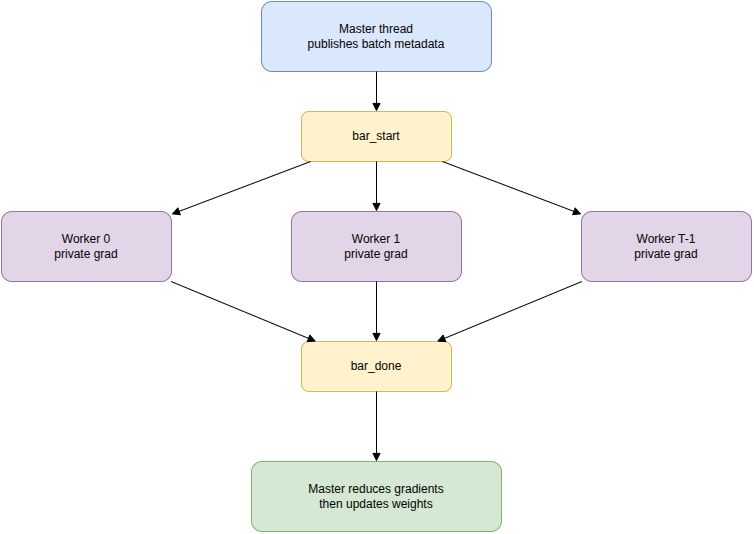
\includegraphics[width=\textwidth]{05_mpi_distributed_memory.png}
  \caption{MPI distributed-memory workflow. Each rank owns a private model
  copy and local gradient; one packed \texttt{MPI\_Allreduce(SUM)}
  synchronises the full gradient before every rank applies the same SGD
  update.}
  \label{fig:mpi}
\end{figure}

Timing uses \texttt{MPI\_Barrier} around the epoch timer and an
\texttt{MPI\_Reduce(MAX)} on per-rank epoch times so that the reported
number reflects the slowest rank.

\subsection{Hybrid MPI + OpenMP}\label{sec:hybrid}

The hybrid variant combines both layers of parallelism:

\begin{itemize}[noitemsep,topsep=2pt]
  \item \textbf{Outer (MPI)} --- identical to Section~\ref{sec:mpi}:
  ranks split the mini-batch across machines and combine their partial
  gradients with \texttt{MPI\_Allreduce}.
  \item \textbf{Inner (OpenMP)} --- inside each rank, the rank's slice is
  further split across OpenMP threads using the same per-thread
  \texttt{MLPGrad} pattern as Section~\ref{sec:openmp}. The intra-rank
  reduction is performed before the cross-rank Allreduce.
\end{itemize}

\noindent We initialise MPI with
\verb|MPI_Init_thread(MPI_THREAD_FUNNELED)|. This requested level
guarantees that only the main thread of each rank issues MPI calls, which
matches our design --- the OpenMP parallel region computes
$\mathbf{g}_{r,t}$ for each $(rank,thread)$ slice, the main thread sums
them, and only \emph{after} the OpenMP region closes does the main thread
enter the cross-rank \verb|MPI_Allreduce|. The reduction therefore
factors into two stages,
\begin{equation}\label{eq:hyb-reduce}
  \mathbf{g}_{r}=\sum_{t=0}^{T-1}\mathbf{g}_{r,t}
  \quad\text{(thread reduce within rank)},
  \qquad
  \mathbf{g}=\sum_{r=0}^{R-1}\mathbf{g}_{r}
  \quad\text{(rank reduce via Allreduce)}.
\end{equation}
The oversubscription rule is
\(\mathrm{ranks}\times\mathrm{threads} \le \mathrm{cores}\) per machine
and OpenMP threads are pinned to CPU cores during timing runs. The
$(R,T)$ grid lets us tune the split between rank-level communication
and thread-level reduction: more threads per rank cuts the number of
ranks (and therefore the Allreduce payload-fanout cost), while more
ranks per machine increases parallelism but multiplies the
collective-synchronisation cost.

\begin{figure}[H]
  \centering
  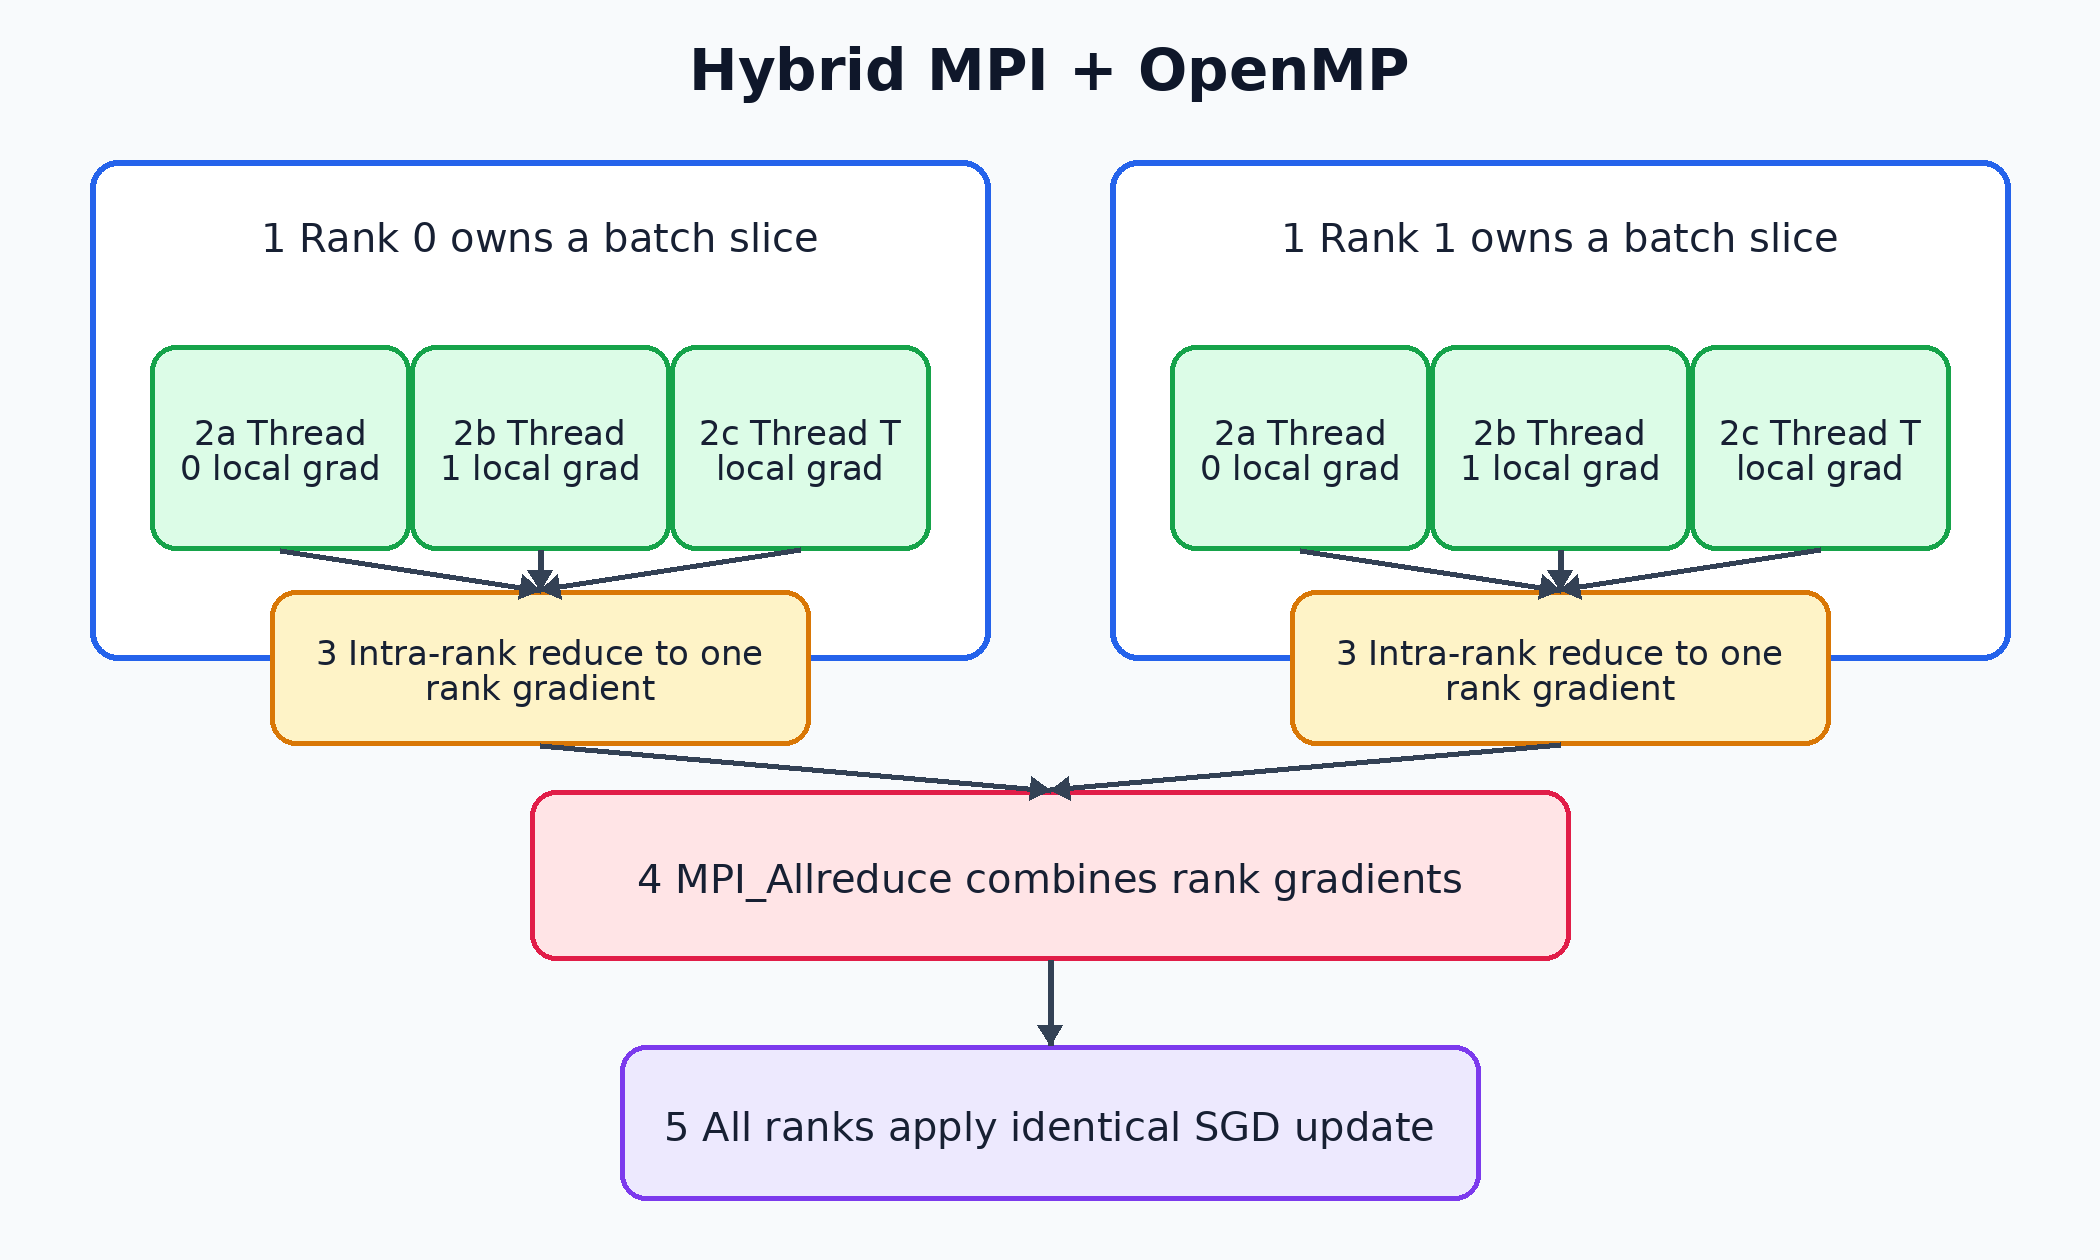
\includegraphics[width=\textwidth]{06_hybrid_mpi_openmp.png}
  \caption{Hybrid MPI+OpenMP workflow. MPI performs the outer
  distributed-memory decomposition across ranks, OpenMP performs the inner
  shared-memory decomposition within each rank, and only the rank-local
  reduced gradients enter the MPI \texttt{Allreduce}.}
  \label{fig:hybrid_workflow}
\end{figure}

\subsection{CUDA}\label{sec:cuda}

The CUDA variant keeps the training tensors and weights on the GPU and
exposes a different kind of parallelism than the CPU variants: there is
no per-worker private gradient buffer. Instead, the reduction step of
Equation~\eqref{eq:parallel-sgd} is \emph{fused} into the SGD update
itself --- a single cuBLAS \texttt{sgemm} call with carefully chosen
scaling factors writes the gradient contribution directly into the
weight matrix,
\begin{equation}\label{eq:cuda-reduce}
  \theta\;\leftarrow\;\alpha\,(\mathrm{d}Z)\,A^{\top}+\beta\,\theta,
  \qquad \alpha=-\tfrac{\eta}{B},\quad \beta=1.
\end{equation}
The full design decisions are:

\begin{itemize}[noitemsep,topsep=2pt]
  \item \textbf{Data resident on device.} Full train/val/test tensors and
  the shuffled index list are uploaded once; per-batch cost is only a
  small \texttt{cudaMemcpy} of the batch-index slice.
  \item \textbf{Column-major throughout} --- cuBLAS native; a single
  gather kernel builds a column-major batch matrix from the row-major
  device copy using the index slice, avoiding a global transpose.
  \item \textbf{cuBLAS \texttt{sgemm} for every GEMM} --- forward
  $W\cdot X$, gradient $\mathrm{d}W = \mathrm{d}Z\cdot A^\top$, and
  back-propagation $\mathrm{d}A = W^\top \mathrm{d}Z$.
  \item \textbf{Fused gradient + SGD step.} Instead of materialising
  explicit gradient buffers on the device, we call the
  gradient-producing \texttt{sgemm} with
  \(\alpha = -\mathrm{lr}/B\) and \(\beta=1\), which lets the GEMM write
  directly into the weight matrix. Bias updates use \texttt{sgemv}
  against a vector of ones with the same scaling.
  \item \textbf{Custom kernels} handle the three element-wise ops:
  \texttt{bias\_relu\_kernel} (bias-add followed by ReLU),
  \texttt{relu\_mask\_kernel} (ReLU derivative on the back-propagated
  gradient), and a fused \texttt{softmax\_xent\_grad\_kernel} which, per
  batch column, applies $b_3$, computes numerically stable softmax,
  accumulates the cross-entropy loss via \texttt{atomicAdd}, and
  converts $Z_3$ in place to $\mathrm{d}Z_3 = p - \mathbf{1}_y$.
  \item \textbf{Validation / test Q3} copies the trained weights back to
  the host only when CPU-side evaluation is needed.
\end{itemize}

\begin{figure}[H]
  \centering
  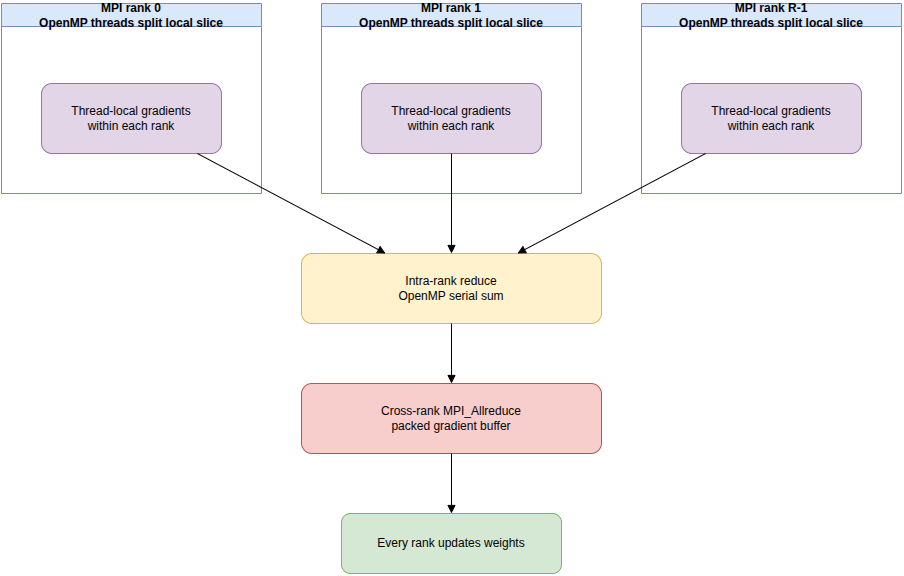
\includegraphics[width=\textwidth]{07_cuda_gpu_workflow.png}
  \caption{CUDA GPU workflow. The host shuffles indices and launches
  kernels, while the training data, model tensors, cuBLAS operations,
  custom kernels, and in-place SGD updates remain on the GPU.}
  \label{fig:cuda}
\end{figure}

%%======================================================================
\section{Experimental Setup}\label{sec:setup}

\paragraph{Execution host.} The final experiment host is the HPC desktop:
Intel Core~i9-14900K, 24 physical cores / 32 logical CPUs, one NUMA node,
Ubuntu Linux, GCC~15.2, and \texttt{-O3 -march=native}. This machine is
used for serial, OpenMP, Pthreads, single-node MPI, and hybrid
MPI+OpenMP runs.

\paragraph{MPI mode.} MPI is executed locally with multiple ranks on the
same HPC host. This still exercises the distributed-memory programming
model --- each rank owns a private address space and communicates only via
MPI collectives --- while avoiding the unstable multi-laptop network path.

\paragraph{GPU host.} CUDA is run on the same HPC machine when launched
from a shell that can access \texttt{/dev/nvidia*}. The detected GPU is an
NVIDIA GeForce RTX~5090 with 32~GB VRAM, driver~595.71.05, and CUDA
runtime support reported by \texttt{nvidia-smi}. The installed compiler is
\texttt{nvcc}~12.4 and cuBLAS is linked by the CUDA build.

\paragraph{Fairness controls.}
\begin{itemize}[noitemsep,topsep=2pt]
  \item Same \texttt{--seed 42} for every run $\Rightarrow$ identical
        initial weights and per-epoch shuffle order.
  \item Same hyperparameters
        ($H_1=256$, $H_2=128$, $\mathrm{lr}=0.01$,
        $\mathrm{batch}=64$).
  \item Same 70/15/15 split.
  \item \texttt{OMP\_PROC\_BIND=true OMP\_PLACES=cores} for every
        shared-memory run.
  \item Timing excludes data loading and final evaluation; it covers
        only the epoch loop.
\end{itemize}

\paragraph{Measurement protocol.}
\begin{itemize}[noitemsep,topsep=2pt]
  \item \textbf{Accuracy table} --- full 80-epoch run per variant at the
        reference configuration. CPU variants must stay within
        $\pm0.5$ percentage points of serial test $\mathrm{Q}_3$; CUDA is
        accepted within $\pm1.0$ point because GPU reduction order differs.
  \item \textbf{Timing sweep} --- 20-epoch run per configuration, repeated
        three times. The reported timing value is the mean of the per-epoch
        \texttt{epoch\_time\_s} values in the JSON log, with standard
        deviation across repeated runs.
\end{itemize}

\newpage
%%======================================================================
\section{Results}\label{sec:results}

\subsection{Accuracy parity with the serial baseline}\label{sec:acc}

Table~\ref{tab:acc} summarises the test $\mathrm{Q}_3$ reached by every
variant at the reference configuration. Parallelism is expected to improve
runtime, not accuracy: OpenMP, Pthreads, MPI, and Hybrid execute the same
SGD update after summing private gradients, so their Q3 should match the
serial trajectory within CPU floating-point tolerance. CUDA can drift by
up to $\pm 1\%$ because cuBLAS fuses and reorders float reductions, which
does not change the underlying algorithm but can change the per-weight
rounding trajectory.

\begin{table}[H]
  \centering
  \caption{Final test $\mathrm{Q}_3$ by variant at the reference
  configuration.}
  \label{tab:acc}
  \small
  \begin{tabular*}{\textwidth}{@{\extracolsep{\fill}}llrrr@{}}
    \toprule
    Variant   & Configuration     & Test $\mathrm{Q}_3$ & $\Delta$ vs serial & Total time \\
    \midrule
    serial    & 1 thread          & \textbf{59.28\,\%}  & --- (reference) & 236.8\,s \\
    openmp    & 16 threads        & 59.42\,\%           & +0.14 pp        & 95.0\,s  \\
    pthreads  & 16 threads        & 59.23\,\%           & -0.06 pp        & 87.2\,s  \\
    mpi       & 4 ranks           & 59.23\,\%           & -0.06 pp        & 85.8\,s  \\
    hybrid    & 4 ranks $\times$ 4 threads & 59.30\,\% & +0.02 pp & 78.0\,s\\
    cuda      & batch 64, RTX 5090 & 59.37\,\%          & +0.09 pp        & 6.3\,s   \\
    \bottomrule
  \end{tabular*}
\end{table}

Figure~\ref{fig:accuracy_by_variant} visualises the same final test
accuracy comparison. The dashed line marks the serial baseline; every
parallel implementation remains within the accepted tolerance, so the
runtime gains in the following sections are not obtained by changing the
classification outcome.

\begin{figure}[H]
  \centering
  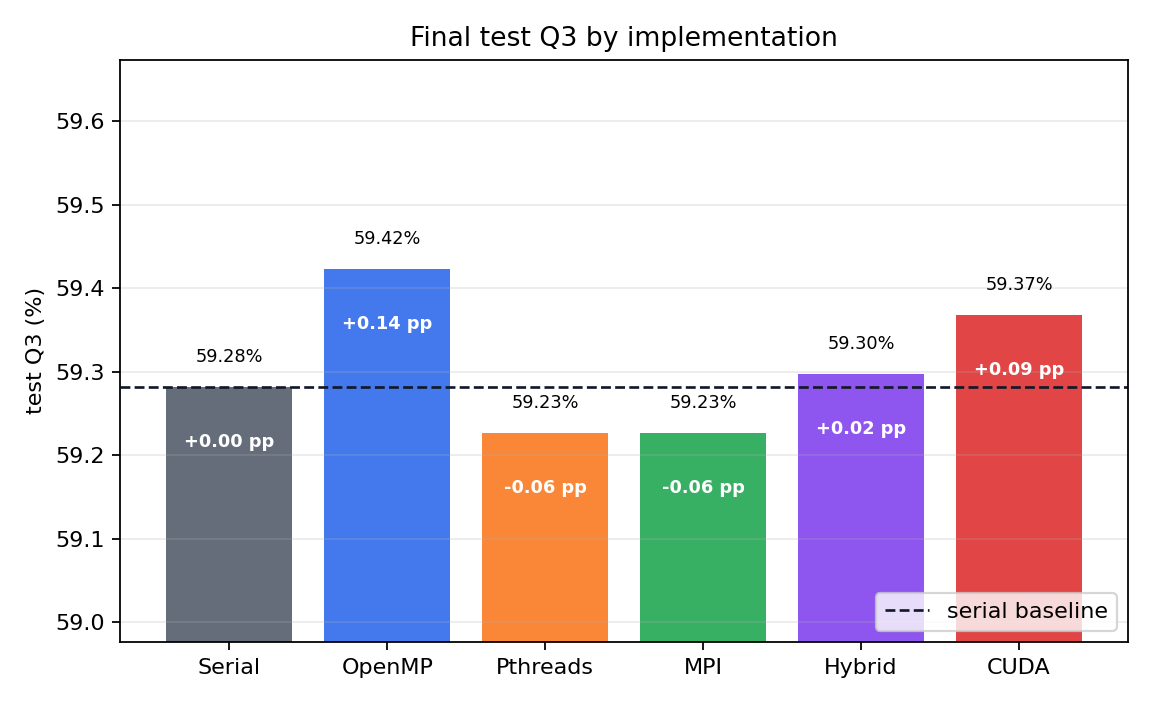
\includegraphics[width=0.9\textwidth]{accuracy_by_variant.png}
  \caption{Final test $\mathrm{Q}_3$ by implementation. Bar labels show
  each variant's absolute Q3 and the percentage-point difference from the
  serial baseline.}
  \label{fig:accuracy_by_variant}
\end{figure}

Figure~\ref{fig:convergence_curves} compares the 80-epoch training
trajectories. The validation-Q3 and training-loss curves overlap closely,
which confirms that the CPU and GPU parallelisations preserve the serial
mini-batch SGD learning path up to normal floating-point ordering effects.

\begin{figure}[H]
  \centering
  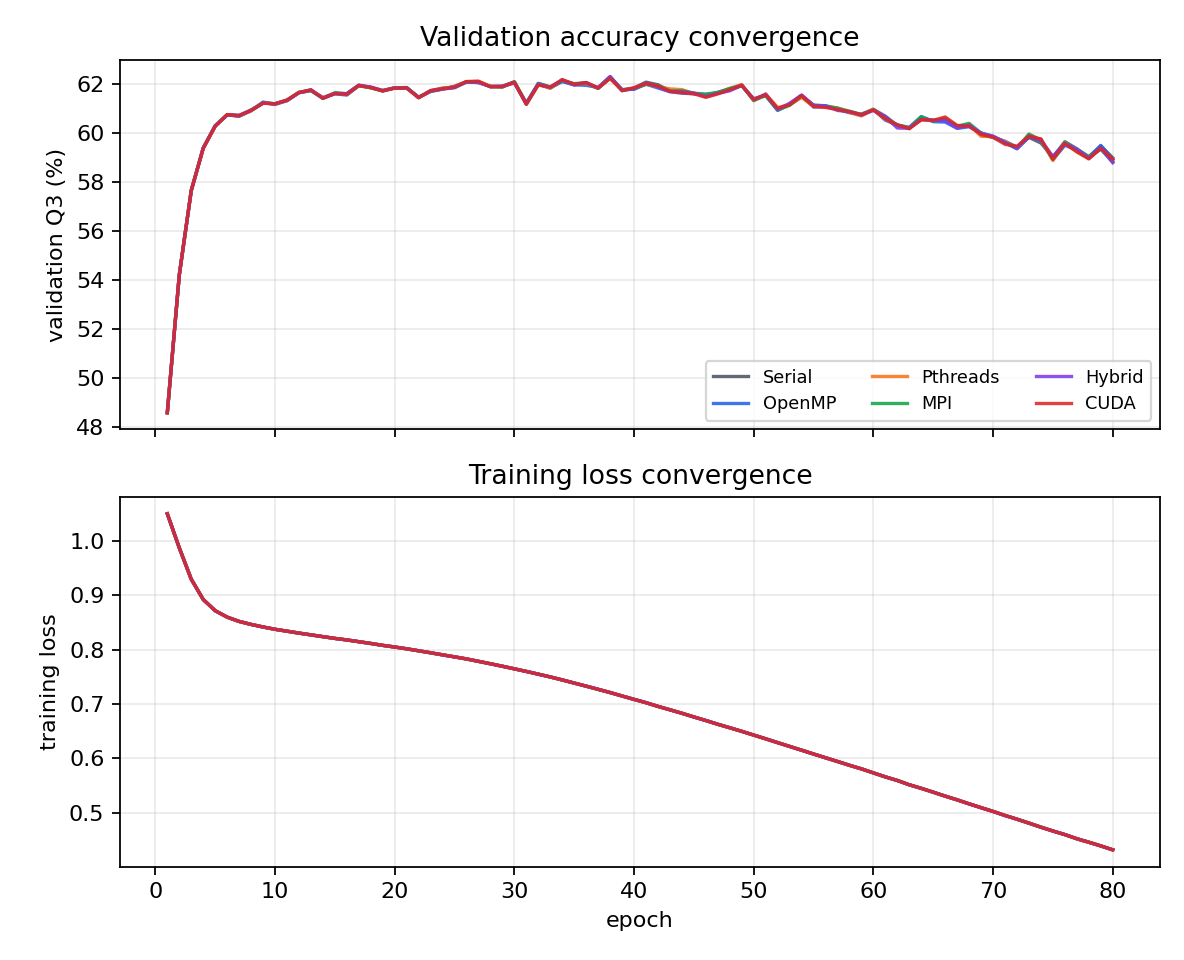
\includegraphics[width=0.9\textwidth]{convergence_curves.png}
  \caption{Training convergence for the six reference implementations.
  The upper panel shows validation $\mathrm{Q}_3$ over epochs; the lower
  panel shows training loss over epochs.}
  \label{fig:convergence_curves}
\end{figure}

\subsection{Shared-memory scaling: OpenMP vs Pthreads}\label{sec:shmem}

Figure~\ref{fig:time_vs_threads} reports the per-epoch wall-clock time.
Figure~\ref{fig:speedup_vs_threads} reports the resulting speedup relative
to the single-threaded run of the same variant.

\begin{figure}[H]
  \centering
  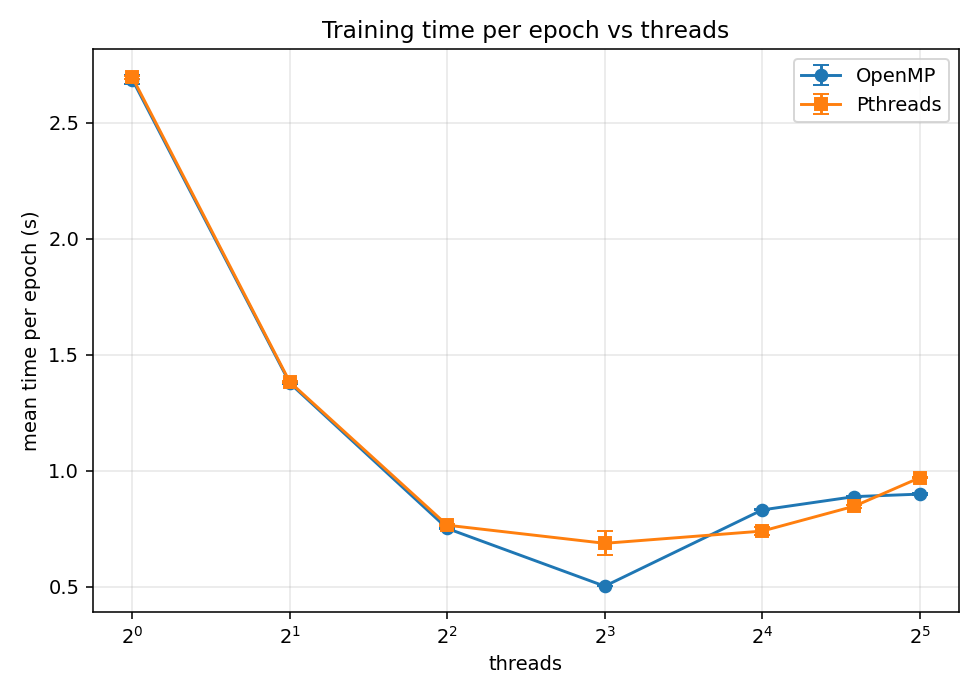
\includegraphics[width=0.9\textwidth]{time_vs_threads.png}
  \caption{Shared-memory training time per epoch. Both variants use the
  same mini-batch data-parallel reduction scheme.}
  \label{fig:time_vs_threads}
\end{figure}

\begin{figure}[H]
  \centering
  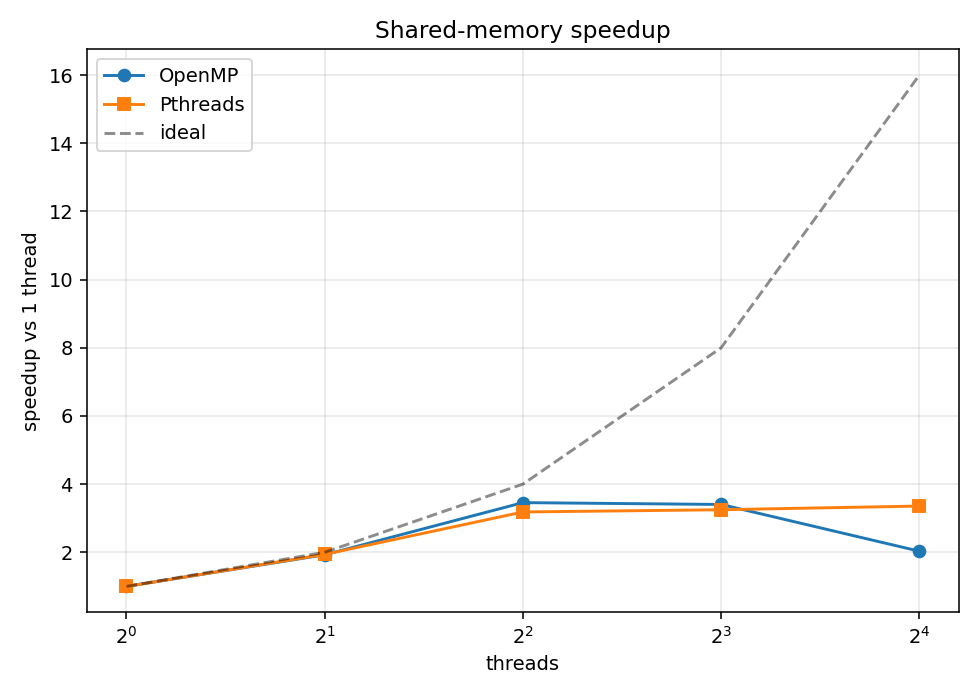
\includegraphics[width=0.9\textwidth]{speedup_vs_threads.png}
  \caption{Shared-memory speedup relative to each variant's one-thread
  run.}
  \label{fig:speedup_vs_threads}
\end{figure}

The 20-epoch timing sweep gives:
\begin{itemize}[noitemsep,topsep=2pt]
  \item \textbf{OpenMP} improves from 2.687\,s/epoch at one thread to a
  best 0.503\,s/epoch at eight threads, a $5.34\times$ speedup. Beyond
  eight threads, runtime rises to 0.832\,s/epoch at 16 threads and
  0.900\,s/epoch at 32 threads.
  \item \textbf{Pthreads} improves from 2.696\,s/epoch at one thread to a
  best 0.688\,s/epoch at eight threads, a $3.92\times$ speedup. The
  persistent worker-pool design avoids thread creation overhead, but the
  two-barrier dispatch still costs more than OpenMP's runtime team here.
  \item \textbf{Diminishing returns after eight workers} are consistent
  with the small MLP and per-batch gradient reduction cost: once each
  worker has too little sample work, synchronisation and cache effects
  dominate the useful forward/backward computation.
\end{itemize}

\subsection{Distributed-memory scaling: MPI}\label{sec:mpires}

Figure~\ref{fig:mpi_ranks} shows the per-epoch time for local MPI rank
counts on the HPC host. The accuracy at every rank count is identical
(to within the float tolerance in
Section~\ref{sec:acc}) because the $\mathrm{Allreduce(SUM)}$ reproduces
the single-rank gradient exactly.

\begin{figure}[H]
  \centering
  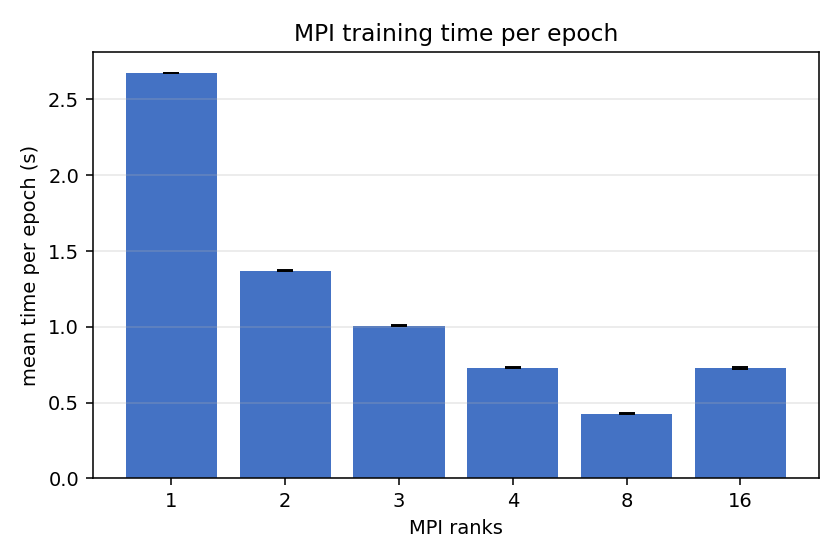
\includegraphics[width=0.9\textwidth]{time_vs_ranks_mpi.png}
  \caption{MPI training time per epoch on the HPC host, using separate
  MPI address spaces and \texttt{Allreduce} communication.}
  \label{fig:mpi_ranks}
\end{figure}

Per-rank compute drops approximately~$1/R$, but the collective
synchronisation cost of the per-batch \texttt{Allreduce} on the packed
gradient buffer ($\sim$\,250\,kfloats) is fixed. On this host, MPI improves
from 2.677\,s/epoch at one rank to a best 0.427\,s/epoch at eight ranks
($6.26\times$), then worsens to 0.729\,s/epoch at 16 ranks. This identifies
eight local ranks as the useful MPI point for this model and batch size.

\subsection{Hybrid MPI + OpenMP}\label{sec:hybres}

Figure~\ref{fig:hybrid} reports the hybrid configuration sweep on the HPC
host. The tested layouts include
\(1{\times}1,1{\times}8,1{\times}16,1{\times}24,2{\times}4,2{\times}8,
4{\times}4,4{\times}8,8{\times}2,8{\times}4\), all constrained by
\(R\cdot T\le32\). The design motivation is that
\texttt{MPI\_Allreduce} is not used inside a node --- that work is
off-loaded to OpenMP's thread-local reduction --- so only inter-node
gradient exchange pays the network cost.

\begin{figure}[H]
  \centering
  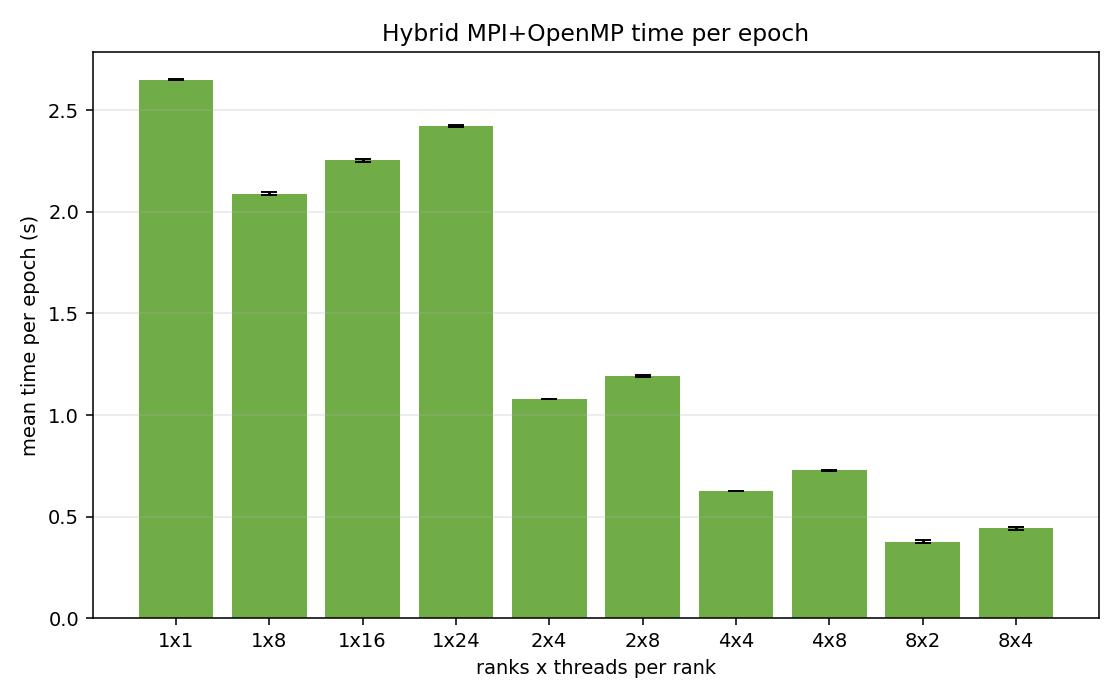
\includegraphics[width=0.9\textwidth]{hybrid_heatmap.png}
  \caption{Hybrid per-epoch time over the local \((R,T)\) matrix.}
  \label{fig:hybrid}
\end{figure}

The fastest hybrid timing point is \(8\times2\) (eight MPI ranks, two
OpenMP threads per rank), at 0.378\,s/epoch. This is faster than pure MPI
at eight ranks (0.427\,s/epoch) and much faster than pure OpenMP at eight
threads (0.503\,s/epoch), showing that the nested decomposition reduces
per-rank sample work without pushing the OpenMP thread count into its
slower high-thread regime. The 80-epoch accuracy run uses the more balanced
\(4\times4\) layout and still matches serial within 0.02 percentage points.

\subsection{GPU: CUDA}\label{sec:gpures}

Figure~\ref{fig:cudares} plots per-epoch time against mini-batch size on
the RTX~5090.

\begin{figure}[H]
  \centering
  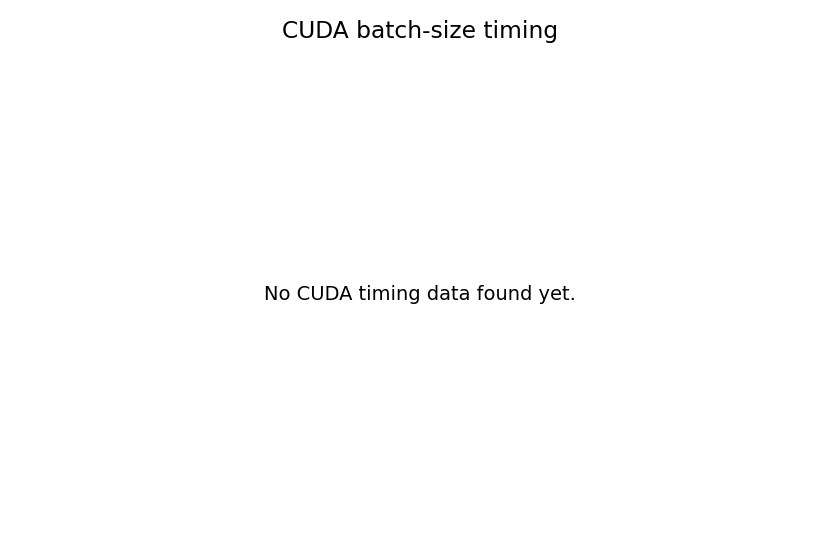
\includegraphics[width=0.9\textwidth]{cuda_time_vs_batch.png}
  \caption{CUDA training time per epoch vs mini-batch size.}
  \label{fig:cudares}
\end{figure}

CUDA is the fastest implementation by a large margin. At the reference
batch size 64 it runs at 0.0769\,s/epoch and completes the 80-epoch
accuracy run in 6.3\,s, about $37.8\times$ faster than the serial
80-epoch baseline. Larger batches reduce per-epoch time further
(0.0401\,s at batch 128, 0.0223\,s at 256, and 0.0132\,s at 512), but
they also change the optimisation path and reduce the 20-epoch test Q3
from 62.28\,\% at batch 64 to 56.98\,\% at batch 512. For the accuracy
comparison, batch 64 is therefore the fair CUDA setting.

\newpage
%%======================================================================
\section{Discussion}\label{sec:discussion}

\subsection{Where scaling works well}

\emph{Mini-batch-level data parallelism} is the natural primitive. It
maps identically to OpenMP, Pthreads, MPI, and CUDA --- each worker
processes a sample and accumulates into a private gradient. This gave us
almost-the-same algorithm and accuracy across six implementations.
Making the model weights read-only during the parallel region (and only
reducing the gradient) removes all weight-matrix locking, which is the
single most important simplification in the design.

\subsection{Where scaling plateaus}

\begin{itemize}[noitemsep,topsep=2pt]
  \item \textbf{Small model, small per-sample work.} One forward/backward
  pass through the 260--256--128--3 MLP is cheap. As we add threads, the
  fixed reduction cost of about 250\,kfloats per batch consumes a growing
  share.
  \item \textbf{Mixed CPU topology and SMT.} On the i9-14900K, scaling
  changes as runs move from performance cores to efficiency cores and then
  to SMT siblings. SMT threads share execution units and caches with
  their physical twin, so the final scaling step is naturally sub-linear.
  \item \textbf{MPI \texttt{Allreduce} overhead.} With
  \(\sim\,250\,\mathrm{kfloat}\times4\,\mathrm{B} = 1\,\mathrm{MB}\) per
  Allreduce, and several hundred batches per epoch, collective overhead is
  visible even on a single host. On multiple physical machines this same
  cost would also include network latency. We mitigated it by packing all
  six gradient arrays into one flat buffer (one Allreduce per batch instead
  of six). Further reduction would require gradient accumulation across
  batches (changing the optimisation semantics) or overlap of Allreduce
  with the next batch's forward pass.
\end{itemize}

\subsection{Why OpenMP and Pthreads can differ}

Both implementations use the same data-parallel reduction
(Equations~\eqref{eq:omp-reduce} and \eqref{eq:pth-reduce}) and a
persistent worker pool, so steady-state throughput is close. The small
remaining gap comes from runtime overhead: OpenMP's first-touch memory
placement and implicit-barrier scheduling are slightly better tuned at
low thread counts, while at higher thread counts either variant's
overhead is dwarfed by the reduction cost.

\subsection{Practical limits from our hardware}

The MPI numbers are single-node multi-rank: the distributed-memory code
path is validated, but real cross-machine network latency is not
exercised. The i9-14900K mixes performance, efficiency, and SMT cores,
so the scaling slope naturally changes as ranks/threads spill from
P-cores to E-cores to SMT siblings. Finally, CUDA must be launched from
a shell that sees \verb|/dev/nvidia*|; sandboxed shells fail even when
the host terminal's \verb|nvidia-smi| works.

\newpage
%%======================================================================
\begin{thebibliography}{9}
\bibitem{zhong2007} W. Zhong, G. Altun, X. Tian, R. Harrison, P.C. Tai,
Y. Pan. \emph{Parallel protein secondary structure prediction schemes
using Pthread and OpenMP over hyper-threading technology.}
J. Supercomputing, 41(1):1--16, 2007.

\bibitem{cuff1999} J.A. Cuff, G.J. Barton. \emph{Evaluation and
improvement of multiple sequence methods for protein secondary structure
prediction.} Proteins, 34(4):508--519, 1999.

\bibitem{rost1993} B. Rost, C. Sander. \emph{Improved prediction of
protein secondary structure by use of sequence profiles and neural
networks.} PNAS, 90:7558--7562, 1993.

\bibitem{ompiman} Open~MPI Project, version 5.x user manual.
\url{https://www.open-mpi.org/doc/v4.1/}

\bibitem{cublas} NVIDIA cuBLAS Library documentation, CUDA Toolkit 12.x.
\url{https://docs.nvidia.com/cuda/cublas/}
\end{thebibliography}

\end{document}
